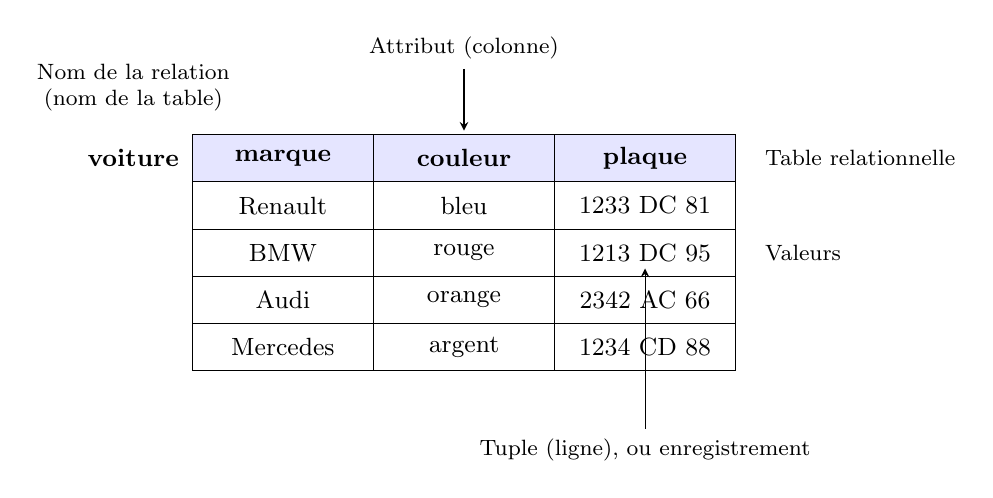
\begin{tikzpicture}[x=1cm,y=1cm,c/.style={draw,minimum height=0.6cm,minimum width=2.3cm,font=\small},h/.style={c,fill=blue!10,font=\small\bfseries},n/.style={font=\footnotesize,align=center,text=black}]
\node[h] at (0.0,0.0){marque};
\node[h] at (2.3,0.0){couleur};
\node[h] at (4.6,0.0){plaque};
\node[c] at (0.0,-0.6){Renault};
\node[c] at (2.3,-0.6){bleu};
\node[c] at (4.6,-0.6){1233 DC 81};
\node[c] at (0.0,-1.2){BMW};
\node[c] at (2.3,-1.2){rouge};
\node[c] at (4.6,-1.2){1213 DC 95};
\node[c] at (0.0,-1.8){Audi};
\node[c] at (2.3,-1.8){orange};
\node[c] at (4.6,-1.8){2342 AC 66};
\node[c] at (0.0,-2.4){Mercedes};
\node[c] at (2.3,-2.4){argent};
\node[c] at (4.6,-2.4){1234 CD 88};
\node[n] (rel) at (-1.9,0.9){Nom de la relation\\(nom de la table)};\node[font=\small\bfseries] at (-1.9,0){voiture};
\node[n] (att) at (2.3,1.4){Attribut (colonne)};\draw[->,>=stealth] (att.south)--(2.3,0.35);
\node[n] (tup) at (4.6,-3.7){Tuple (ligne), ou enregistrement};\draw[->,>=stealth] (tup.north)--(4.6,-1.4);
\node[n,anchor=west] at (6.0,-1.2){Valeurs};\node[n,anchor=west] at (6.0,0){Table relationnelle};
\end{tikzpicture}